\documentclass{article}
\usepackage{fullpage}

%load needed packages
\usepackage{graphicx}
\usepackage{array}
\usepackage{booktabs}
\usepackage[utf8]{inputenc}
\usepackage[T1]{fontenc}
\usepackage{hyperref}

\usepackage[spanish]{babel} % Paquete para el idioma español
\usepackage{float}  % Necesario para [H]
\usepackage{listings}
\usepackage{xcolor}
\usepackage{longtable} 

\definecolor{codegreen}{HTML}{5AB2FF}
\definecolor{morado}{HTML}{AD88C6}
\definecolor{BG}{HTML}{EEEEEE}
\definecolor{azul}{HTML}{4D869C}
\definecolor{sqlblue}{HTML}{FF8C00} % Color para las palabras clave SQL

% Estilo para DDL
\lstdefinestyle{ddlstyle}{
	language=SQL,
	backgroundcolor=\color{BG},
	commentstyle=\color{codegreen},
	basicstyle=\ttfamily\small,
	keywordstyle=\color{azul},
	stringstyle=\color{morado},
	showstringspaces=false,
	breaklines=true,
	frame=shadowbox,
	numbers=left,
	numberstyle=\tiny\color{gray},
	captionpos=b,
}

% Estilo para SQL
\lstdefinestyle{sqlstyle}{
	language=SQL,
	backgroundcolor=\color{BG},
	commentstyle=\color{codegreen},
	basicstyle=\ttfamily\small,
	keywordstyle=\color{sqlblue}, % Color diferente para palabras clave SQL
	stringstyle=\color{morado},
	showstringspaces=false,
	breaklines=true,
	frame=shadowbox,
	numbers=left,
	numberstyle=\tiny\color{gray},
	captionpos=b,
}

\begin{document}
	
	% Portada
	\begin{titlepage}
		\centering
		\vspace*{3cm}
		
		% Título destacado
		{\Huge \textbf{Plataforma Web de Rehabilitación a Distancia}\\[0.5cm]}
		
		{\Large \textbf{Entrega Modelado  Draft 1}\\[0.5cm]}
		
		% Espacio y logotipo (si lo tienes, por ejemplo el logo de tu universidad)
		\vspace{2cm}
		
\includegraphics[width=0.3\textwidth]{images/uma_logo.jpg}\\[1cm]
		
		% Nombre del autor
		{\LARGE \textbf{Organización basada en componentes}\\[0.5cm]}
		{\large \textit{Integrantes:}\\
			Cuevas Rodríguez, Marta\\
			de Pablo, Diego\\
			Silva Rodríguez, Alejandro\\
			Soriano Muñoz, Juan Ignacio\\
		}
		\vfill
		{\large \textit{Ingeniería web}\\
			Universidad de Málaga\\
		}
		
		\vfill
		
		% Fecha en la parte inferior de la página
		{\large Octubre 2024}
	\end{titlepage}
	
	% índice
	\tableofcontents
	
	\newpage
	
	\section{Introducción}

La rehabilitación es una fase crítica en el proceso de recuperación de pacientes que han sufrido lesiones, intervenciones quirúrgicas o padecen enfermedades crónicas. Tradicionalmente, la rehabilitación se realiza de manera presencial, lo que puede generar barreras logísticas, económicas y geográficas tanto para los pacientes como para los profesionales de la salud. Ante esta realidad, surge la necesidad de una Plataforma Web de Rehabilitación a Distancia, cuyo objetivo es facilitar el acceso a programas de rehabilitación personalizados, ofrecer seguimiento remoto y mejorar la calidad de vida de los pacientes sin la necesidad de visitas constantes a centros de rehabilitación.
\\
\\
Este proyecto plantea el desarrollo de una plataforma web integral que permita a los pacientes recibir tratamientos de rehabilitación de manera remota, mientras que los profesionales de la salud pueden monitorizar el progreso y ajustar las terapias en tiempo real. Los principales stakeholders involucrados en este proyecto incluyen a pacientes, profesionales de la salud (fisioterapeutas, médicos rehabilitadores) y desarrolladores de software. Los pacientes se beneficiarán de un acceso más flexible a sus tratamientos, mientras que los profesionales podrán optimizar el seguimiento clínico y ajustar terapias de manera eficiente.
\\
\\
Entre los posibles casos de uso se encuentran situaciones como la rehabilitación de un paciente con una lesión muscular, que puede realizar sus ejercicios desde casa bajo la supervisión de un fisioterapeuta a través de videollamadas, o un paciente crónico que, mediante dispositivos de telemetría y un registro de ejercicios, permite que su progreso sea monitorizado de forma continua.


\section{Modelado}



\subsection{Diagrama de Casos de Uso}

Un Diagrama de Casos de Uso muestra las operaciones que se esperan de un sistema y cómo interactúan los usuarios u otros sistemas con él. Es una herramienta esencial para la planificación y control de proyectos interactivos, permitiendo una visión clara de los requisitos que debe cumplir el sistema.

Cada caso de uso se representa mediante una elipse que denota una operación completa desarrollada entre el sistema y sus actores. El conjunto de casos de uso refleja la totalidad de las operaciones realizadas por el sistema.

Otros elementos que serán visto en el diagrama de casos de uso (ver figura \ref{fig:requisitos_diagrama})

\begin{itemize}
	\item \textbf{Actor}: Es un usuario del sistema que interactúa con uno o más casos de uso. Un actor puede representar tanto a personas como a sistemas externos que necesitan acceder a información o servicios del sistema. Un actor puede tener múltiples roles, y un caso de uso puede tener varios actores.
	
	\item \textbf{Generalización de Actor}: Permite agrupar actores con comportamientos similares. Por ejemplo, un \textit{Usuario} puede ser una generalización de \textit{Paciente} y \textit{Profesional de la salud}, dado que ambos comparten ciertas acciones comunes, pero también tienen roles específicos.
	
	\item \textbf{Relaciones Especiales}:
	\begin{itemize}
		\item \textbf{Uses}: Denota la inclusión del comportamiento de un caso de uso en otro. Se utiliza cuando el comportamiento es compartido entre varios casos de uso.
		\item \textbf{Extends}: Indica una especialización de un caso de uso base. Se utiliza cuando un comportamiento adicional o alternativo se activa bajo ciertas condiciones.
	\end{itemize}
\end{itemize}

\begin{figure}[h!]
	\begin{center} 
		\includegraphics[width=1\textwidth]{images/Casos_de_uso_rehabilitación.jpg}
		\caption{Diseño de Diagrama de Casos de Uso}
		\label{fig:requisitos_diagrama}
	\end{center}
\end{figure}

\subsection{Explicación de Casos de Uso}

\subsubsection*{CASO DE USO 1: Paciente registrando sus resultados}

\begin{itemize}
	\item \textbf{Nombre}: Registrar resultados del paciente.
	\item \textbf{Objetivo}: El paciente registra sus resultados de la rutina de ejercicios.
	\item \textbf{Autor}: Paciente
	\item \textbf{Descripción}: 
	El paciente, que ya está registrado en la aplicación, inicia sesión correctamente y accede al espacio de progreso. Si el paciente utiliza sensores o dispositivos Wearables, estos se conectarán automáticamente para introducir datos de actividad física y otras métricas. Además, el paciente podrá responder preguntas sobre su comodidad con la rutina, sus preferencias, y su estado de salud general. Si el paciente completa su rutina de ejercicios, la aplicación puede desbloquear logros (gamificación) como incentivo para continuar.
\end{itemize}

\textbf{Precondiciones:}
\begin{itemize}
	\item El paciente está registrado en la aplicación.
	\item El paciente cuenta con un plan de rehabilitación activo.
	\item El paciente puede disponer de un dispositivo Wearable y conexión a internet adecuada.
\end{itemize}

\textbf{Escenario principal:}
\begin{enumerate}
	\item El paciente abre la página web.
	\item El paciente inicia sesión correctamente.
	\item La página web verifica las credenciales y confirma el inicio de sesión.
	\item El paciente hace clic en el botón \textit{Progreso}.
	\item La página web carga la pestaña de progreso y logros.
	\item El paciente comienza a introducir sus avances en la plataforma.
	\begin{itemize}
		\item Si el paciente tiene un dispositivo Wearable, este carga automáticamente los datos de actividad en su progreso.
	\end{itemize}
	\item La aplicación guarda los datos introducidos.
	\item La aplicación otorga un logro al paciente por cumplir su cuota de actividad.
\end{enumerate}

\textbf{Escenario alternativo:}
\begin{itemize}
	\item En el caso de que el paciente no haya logrado su cuota de actividad, la aplicación no otorgará un logro.
	\item El paciente recibirá un mensaje de motivación para fomentar una mayor actividad física.
\end{itemize}


\subsubsection*{CASO DE USO 2: Pactar una cita con un paciente}

\begin{itemize}
	\item \textbf{Nombre}: Pactar una cita con un paciente
	\item \textbf{Objetivo}: El profesional de la salud programa una cita de seguimiento con un paciente.
	\item \textbf{Autor}: Profesional de la salud
	\item \textbf{Descripción}: 
	El profesional de la salud, después de iniciar sesión correctamente, selecciona un paciente de su lista de pacientes. El profesional puede revisar la disponibilidad del paciente y programar una cita de seguimiento, ya sea en persona o por videollamada, para continuar con el plan de rehabilitación. La cita se agenda en el calendario del paciente, y ambos reciben una notificación automática.
\end{itemize}

\textbf{Precondiciones:}
\begin{itemize}
	\item El profesional de la salud está registrado en la plataforma y ha iniciado sesión.
	\item El paciente está registrado en la plataforma y tiene un plan de rehabilitación activo.
	\item El paciente tiene habilitado el acceso a su calendario para recibir notificaciones.
\end{itemize}

\textbf{Escenario principal:}
\begin{enumerate}
	\item El profesional de la salud abre la página web.
	\item El profesional inicia sesión correctamente.
	\item La página web verifica las credenciales y confirma el inicio de sesión.
	\item El profesional selecciona un paciente de la lista.
	\item El profesional hace clic en la opción \textit{Pactar cita}.
	\item La plataforma muestra el calendario del paciente con las franjas horarias disponibles.
	\item El profesional selecciona una fecha y hora para la cita.
	\item La plataforma confirma la cita y la agenda en el calendario del paciente.
	\item Se envía una notificación automática al paciente y al profesional.
\end{enumerate}

\textbf{Escenario alternativo:}
\begin{itemize}
	\item Si no hay disponibilidad en el calendario del paciente, la plataforma notifica al profesional y sugiere nuevas franjas horarias.
	\item Si el paciente cancela la cita, la plataforma envía una notificación al profesional para reprogramar.
\end{itemize}

\subsubsection*{CASO DE USO 3: Modificar plan de rehabilitación de un paciente}

\begin{itemize}
	\item \textbf{Nombre}: Modificar plan de rehabilitación de un paciente
	\item \textbf{Objetivo}: El profesional de la salud modifica el plan de rehabilitación de un paciente.
	\item \textbf{Autor}: Profesional de la salud
	\item \textbf{Descripción}: 
	El profesional de la salud selecciona un paciente de su lista y revisa su progreso. Basado en el desempeño y las necesidades actuales del paciente, el profesional decide modificar el plan de rehabilitación existente. Esto puede implicar ajustar la rutina de ejercicios, cambiar la frecuencia de sesiones o actualizar las metas de recuperación. Una vez modificado, el nuevo plan es guardado y notificado al paciente.
\end{itemize}

\textbf{Precondiciones:}
\begin{itemize}
	\item El profesional de la salud está registrado en la plataforma y ha iniciado sesión.
	\item El paciente tiene un plan de rehabilitación activo.
	\item El profesional tiene acceso al historial de progreso del paciente.
\end{itemize}

\textbf{Escenario principal:}
\begin{enumerate}
	\item El profesional de la salud abre la página web.
	\item El profesional inicia sesión correctamente.
	\item La página web verifica las credenciales y confirma el inicio de sesión.
	\item El profesional selecciona un paciente de la lista.
	\item El profesional hace clic en la opción \textit{Modificar plan de rehabilitación}.
	\item La plataforma muestra el plan de rehabilitación actual del paciente.
	\item El profesional realiza modificaciones al plan (ej. ajustar ejercicios, cambiar frecuencia, actualizar metas).
	\item El profesional guarda las modificaciones.
	\item La plataforma envía una notificación al paciente informando los cambios en su plan.
\end{enumerate}

\textbf{Escenario alternativo:}
\begin{itemize}
	\item Si el profesional no está seguro de los cambios, puede optar por guardar un borrador del nuevo plan y continuar más tarde.
	\item Si el paciente no está de acuerdo con las modificaciones, puede enviar un mensaje al profesional para discutir los ajustes.
\end{itemize}


\subsection{Diagrama de Secuencia}

Un diagrama de secuencia muestra la interacción de un conjunto de objetos de una aplicación a lo largo del tiempo. Es una herramienta importante porque aporta detalles a los casos de uso, aclarando cómo se intercambian mensajes entre los objetos. Además, revela cómo las clases diseñadas interactúan en el contexto de una operación específica.

Este tipo de diagrama es esencial para comprender la dinámica del sistema en términos de secuencia temporal, permitiendo visualizar el orden en que los mensajes se envían entre objetos y cómo se desarrollan las operaciones en el sistema. Detalla la lógica de las interacciones y ayuda a verificar que el diseño satisface los requisitos funcionales descritos en los casos de uso.

Elementos principales en Visual Paradigm (ver Figura \ref{fig:secuencia_diagrama}):
\begin{itemize}
	\item \textbf{Línea de vida (lifeline)}: Representa la existencia de un objeto a lo largo del tiempo, y se dibuja como una línea vertical punteada con un rectángulo de encabezado.
	\item \textbf{Activación}: Denotada por un rectángulo a lo largo de la línea de vida, representa el periodo en el cual un objeto está ejecutando una operación.
	\item \textbf{Mensaje}: Los mensajes entre objetos se representan mediante líneas sólidas con flechas, que indican el flujo de información desde el objeto que emite el mensaje hasta el objeto que lo recibe y ejecuta.
\end{itemize}

\begin{figure}[h!]
	\begin{center} 
		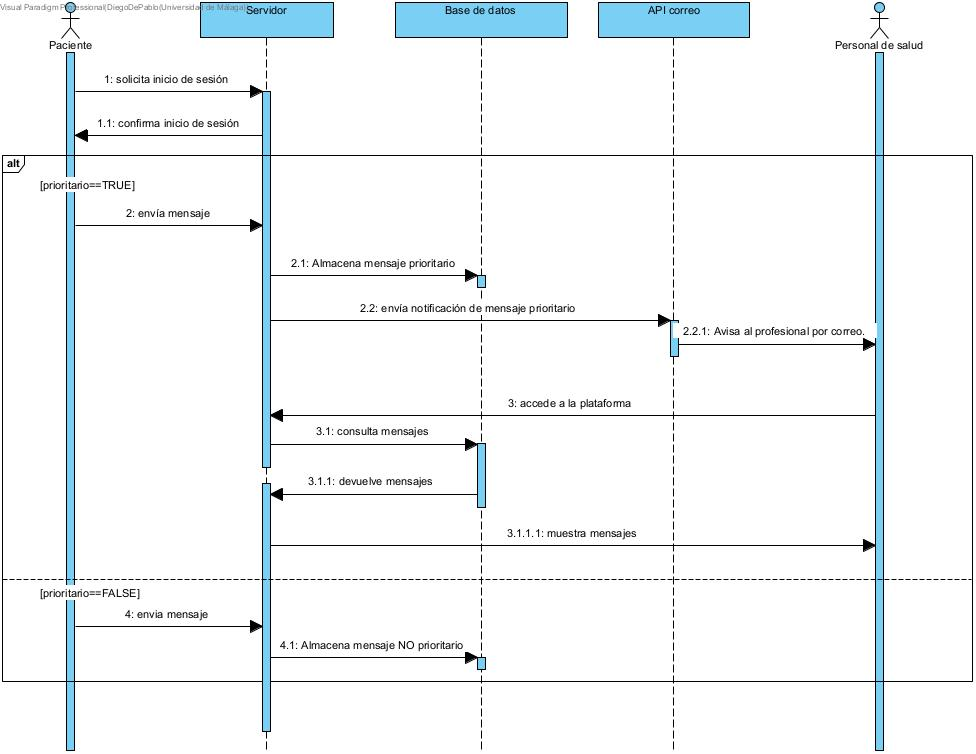
\includegraphics[width=1\textwidth]{images/Diagrama_de_secuencia_rehabilitacion.jpg}
		\caption{Diseño de Diagrama de Secuencia: Paciente envía un mensaje}
		\label{fig:secuencia_diagrama}
	\end{center}
\end{figure}

\subsubsection{Diagrama de Secuencias: Envío de mensaje}

En este apartado, se ha seleccionado un caso de uso particular para detallar la interacción entre las diferentes entidades involucradas en el proceso de \textbf{envío de un mensaje prioritario} por parte del paciente a su profesional de la salud. Este enfoque se eligió para profundizar en las interacciones sin caer en la redundancia con otros diagramas. El caso de uso describe cómo el paciente puede optar por enviar un mensaje marcado como \textit{prioritario}, lo que genera una notificación adicional por correo al profesional, además de ser almacenado en el buzón de alertas.

\textbf{Clases involucradas (lifelines/actores)}:
\begin{itemize}
	\item \textbf{Paciente}: Inicia el flujo al redactar y enviar el mensaje a través de la aplicación.
	\item \textbf{Servidor de la aplicación}: Recibe la solicitud del paciente, almacena el mensaje y gestiona las notificaciones.
	\item \textbf{Base de datos}: Se encarga de almacenar los mensajes enviados y gestionar las alertas en el buzón.
	\item \textbf{Servidor de correo}: Es el encargado de enviar una notificación por correo electrónico al profesional si el mensaje es marcado como prioritario.
	\item \textbf{Profesional de la salud}: El destinatario del mensaje, quien accede a la plataforma para leer el mensaje.
\end{itemize}

\textbf{Secuencia de Interacciones}:
\begin{itemize}
	\item \textbf{Paciente → Iniciar sesión} (\texttt{IniciarSesion(String: usuario, String: contraseña)}): El paciente solicita iniciar sesión en la aplicación para acceder a sus funcionalidades, proporcionando sus credenciales (usuario y contraseña).
	\item \textbf{Servidor de la aplicación → Verificación de credenciales} (\texttt{Verificación(String: usuario, String: contraseña)}): El servidor de la aplicación valida las credenciales consultando la base de datos para confirmar la autenticidad de los datos.
	\item \textbf{Servidor de la aplicación → Login exitoso} (\texttt{Login(Boolean: correcto)}): El servidor responde con un valor booleano, confirmando si las credenciales son correctas (\texttt{true}) o incorrectas (\texttt{false}). En caso positivo, el paciente accede a la interfaz de usuario.
\end{itemize}

\textbf{Redacción y envío del mensaje}:
\begin{itemize}
	\item \textbf{Paciente → Servidor de la aplicación} (\texttt{EnviarMensaje(String: mensaje, Boolean: prioritario)}): El paciente redacta el mensaje y lo envía al servidor, seleccionando si es prioritario o no. El mensaje se transmite junto con un parámetro booleano que indica la prioridad.
	\item \textbf{Servidor de la aplicación → Base de datos} (\texttt{AlmacenarMensaje(String: mensaje)}): El servidor almacena el mensaje en la base de datos, junto con la etiqueta de prioridad si corresponde.
	\item \textbf{Servidor de la aplicación → Profesional de la salud} (\texttt{NotificarMensaje()}): Si el mensaje no es prioritario, el servidor notifica al profesional a través de la plataforma, almacenando el mensaje en el buzón de alertas.
	\item \textbf{Servidor de la aplicación → Servidor de correo} (\texttt{EnviarCorreoNotificacion()}): En el caso de que el mensaje sea prioritario, el servidor también envía una notificación por correo electrónico al profesional a través del servidor de correo.
\end{itemize}

\textbf{Lectura del mensaje por el profesional}:
\begin{itemize}
	\item \textbf{Profesional de la salud → Servidor de la aplicación} (\texttt{ConsultarMensajes()}): El profesional accede a la plataforma y solicita la lista de mensajes.
	\item \textbf{Servidor de la aplicación → Base de datos} (\texttt{RecuperarMensajes()}): El servidor consulta los mensajes almacenados en la base de datos para ese profesional.
	\item \textbf{Base de datos → Servidor de la aplicación} (\texttt{DevolverMensajes()}): La base de datos devuelve los mensajes solicitados.
	\item \textbf{Servidor de la aplicación → Profesional de la salud} (\texttt{MostrarMensajes()}): El servidor muestra los mensajes al profesional, quien puede proceder a leerlos y responder si es necesario.
\end{itemize}

\textbf{Escenarios alternativos}:
El diagrama incluye un bloque condicional (\textit{alt}) que refleja los dos escenarios posibles:
\begin{itemize}
	\item Si el mensaje es \textbf{prioritario}, el profesional recibe una notificación adicional por correo.
	\item Si el mensaje no es prioritario, simplemente se almacena en el buzón de alertas del profesional.
\end{itemize}


\subsection{Diagrama de requisitos en  SysML}

El Diagrama de Requisitos en SysML es una herramienta visual utilizada para documentar y mostrar las relaciones entre los distintos requisitos de un sistema y su trazabilidad. Su objetivo principal es facilitar la comprensión de cómo los requisitos están interconectados y asegurar que se gestionen de manera adecuada durante todo el ciclo de vida del sistema. A través de este diagrama, se pueden identificar relaciones como dependencias, derivaciones o refinamientos entre requisitos, lo que ayuda a los equipos a garantizar que todos los aspectos del sistema estén cubiertos y alineados con los objetivos y restricciones establecidos.
\\

En la figura \ref{fig:SysML} se muestran las diferentes relaciones entre los requisitos funcionales y no funcionales de nuestro sistema.

\begin{figure}
	\begin{center} 
		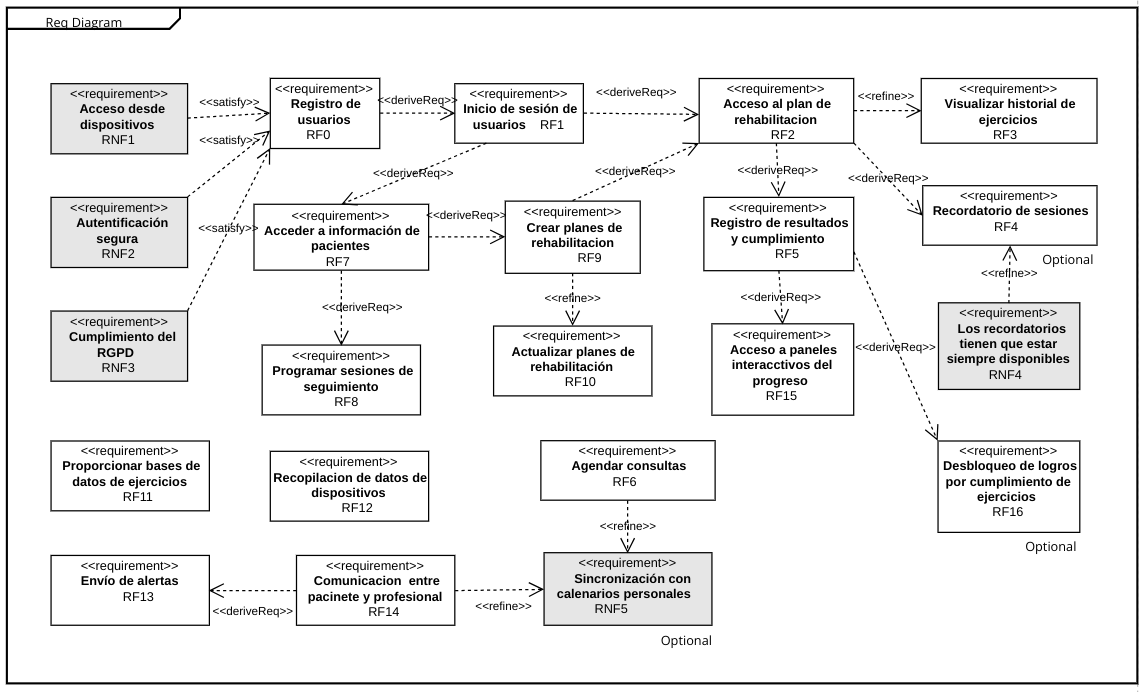
\includegraphics[width=1\textwidth]{images/SysML.png}
		\caption{Diseño de Diagrama de requisitos en SysML}
		\label{fig:SysML}
	\end{center}
\end{figure}
\vspace{5cm}

\subsubsection{Tipos de relaciones}
En el esquema se describen tres tipos de relaciones diferentes.

\begin{itemize}
	\item \textbf{Derivación ("deriveReqt"):} Un requisito se deriva de otro, es decir, el segundo requisito es una consecuencia directa del primero.
	\item \textbf{Satisfacción ("satisfy"):} Un requisito no funcional satisface o cumple con un requisito funcional, indicando que ese aspecto técnico o de comportamiento es necesario para su implementación.
	\item \textbf{Refinamiento ("refine"):} Un requisito refina otro, añadiendo más detalles o especificaciones para clarificar o profundizar en cómo se debe cumplir el requisito original.
\end{itemize}

\subsubsection{Requisitos Principales y sus Relaciones}
\begin{enumerate}
	\item \textbf{RNF1 - Acceso desde dispositivos} \textit{satisface} a \textbf{RF0 - Registro de usuarios}.
	\begin{itemize}
		\item El requisito no funcional RNF1 indica que el sistema debe ser accesible desde distintos dispositivos, lo que satisface el requisito \textbf{Registro de usuarios}, ya que los usuarios deben poder registrarse sin importar el dispositivo.
	\end{itemize}
	
	\item \textbf{RNF2 - Autenticación segura} \textit{satisface} a \textbf{RF0 - Registro de usuarios}.
	\begin{itemize}
		\item El requisito de autenticación segura satisface el requisito de \textbf{Registro de usuarios}, ya que el proceso de registro debe ser seguro para proteger la información de los usuarios.
	\end{itemize}
	
	\item \textbf{RNF2 - Autenticación segura} \textit{satisface} a \textbf{RF7 - Acceder a información de pacientes}.
	\begin{itemize}
		\item La autenticación segura satisface el acceso a la información de los pacientes, asegurando que solo los usuarios autorizados puedan acceder a dicha información.
	\end{itemize}
	
	\item \textbf{RF0 - Registro de usuarios} \textit{derivaReqt} a \textbf{RF1 - Inicio de sesión de usuarios}.
	\begin{itemize}
		\item El inicio de sesión se deriva del \textbf{Registro de usuarios}, ya que solo un usuario registrado podrá iniciar sesión en el sistema.
	\end{itemize}
	
	\item \textbf{RF1 - Inicio de sesión de usuarios} \textit{derivaReqt} a \textbf{RF2 - Acceso al plan de rehabilitación}.
	\begin{itemize}
		\item El acceso a los planes de rehabilitación se deriva del \textbf{Inicio de sesión de usuarios}, ya que solo un usuario autenticado podrá acceder a su plan.
	\end{itemize}
	
	\item \textbf{RF2 - Acceso al plan de rehabilitación} \textit{refine} a \textbf{RF3 - Visualizar historial de ejercicios}.
	\begin{itemize}
		\item El acceso al historial de ejercicios refina el requisito de \textbf{Acceso al plan de rehabilitación}, proporcionando detalles adicionales sobre qué información específica se puede ver en los planes.
	\end{itemize}
	
	\item \textbf{RF2 - Acceso al plan de rehabilitación} \textit{derivaReqt} a \textbf{RF5 - Registro de resultados y cumplimiento}.
	\begin{itemize}
		\item El registro de resultados y cumplimiento deriva del \textbf{Acceso al plan de rehabilitación}, ya que los pacientes deben poder registrar su progreso relacionado con el plan.
	\end{itemize}
	
	\item \textbf{RF3 - Visualizar historial de ejercicios} \textit{refine} a \textbf{RF4 - Recordatorio de sesiones}.
	\begin{itemize}
		\item El recordatorio de sesiones refina el \textbf{Historial de ejercicios}, ya que los recordatorios son una función adicional del sistema que ayuda a los pacientes a seguir sus planes de ejercicios.
	\end{itemize}
	
	\item \textbf{RF4 - Recordatorio de sesiones} \textit{refine} a \textbf{RNF4 - Los recordatorios tienen que estar siempre disponibles}.
	\begin{itemize}
		\item \textbf{Los recordatorios tienen que estar siempre disponibles} refina el \textbf{Recordatorio de sesiones} al indicar que los recordatorios deben estar disponibles 24/7, asegurando que los pacientes reciban esta información en cualquier momento.
	\end{itemize}
	
	\item \textbf{RF5 - Registro de resultados y cumplimiento} \textit{derivaReqt} a \textbf{RF16 - Desbloqueo de logros por cumplimiento de ejercicios}.
	\begin{itemize}
		\item El desbloqueo de logros se deriva del \textbf{Registro de resultados y cumplimiento}, ya que los logros solo se pueden desbloquear una vez que los resultados están registrados y se ha demostrado el cumplimiento del plan.
	\end{itemize}
	
	\item \textbf{RF5 - Registro de resultados y cumplimiento} \textit{derivaReqt} a \textbf{RF15 - Acceso a paneles interactivos del progreso}.
	\begin{itemize}
		\item El acceso a paneles interactivos del progreso se deriva del \textbf{Registro de resultados}, ya que los datos registrados deben estar disponibles para su visualización en los paneles interactivos.
	\end{itemize}
	
	\item \textbf{RF7 - Acceder a información de pacientes} \textit{derivaReqt} a \textbf{RF9 - Crear planes de rehabilitación}.
	\begin{itemize}
		\item La creación de planes de rehabilitación se deriva del \textbf{Acceso a la información de los pacientes}, ya que los profesionales necesitan estos datos para diseñar planes personalizados.
	\end{itemize}
	
	\item \textbf{RF9 - Crear planes de rehabilitación} \textit{refine} a \textbf{RF10 - Actualizar planes de rehabilitación}.
	\begin{itemize}
		\item La actualización de los planes refina la \textbf{Creación de planes}, especificando que los planes pueden y deben ser actualizados a lo largo del tiempo.
	\end{itemize}
	
	\item \textbf{RF6 - Agendar consultas} \textit{refine} a \textbf{RNF5 - Sincronización con calendarios personales}.
	\begin{itemize}
		\item \textbf{Sincronización con calendarios personales} refina la \textbf{Función de agendar consultas}, proporcionando más detalles sobre cómo deben integrarse estas consultas con los calendarios de los usuarios.
	\end{itemize}
	
	\item \textbf{RF13 - Envío de alertas} \textit{derivaReqt} a \textbf{RF14 - Comunicación entre paciente y profesional}.
	\begin{itemize}
		\item La \textbf{Comunicación entre paciente y profesional} se deriva del \textbf{Envío de alertas}, ya que estas alertas pueden generar interacciones directas entre el paciente y el profesional.
	\end{itemize}
	
	\item \textbf{Proporcionar bases de datos de ejercicios} y \textbf{Recopilación de datos de dispositivos}
	\begin{itemize}
		\item Estos requisitos están aislados y no tienen conexiones directas con otros requisitos, lo cual indica que son funcionalidades independientes dentro del sistema.
	\end{itemize}
\end{enumerate}

\newpage
\subsection{Diagrama IFML}


En esta subsección, se describe el uso del lenguaje de modelado IFML (Interaction Flow Modeling Language) en el diseño de la plataforma. IFML se utiliza para modelar las interacciones y flujos de usuario dentro de la aplicación, lo que permite representar visualmente los diferentes escenarios de uso.

\begin{figure}[H]
	\centering
	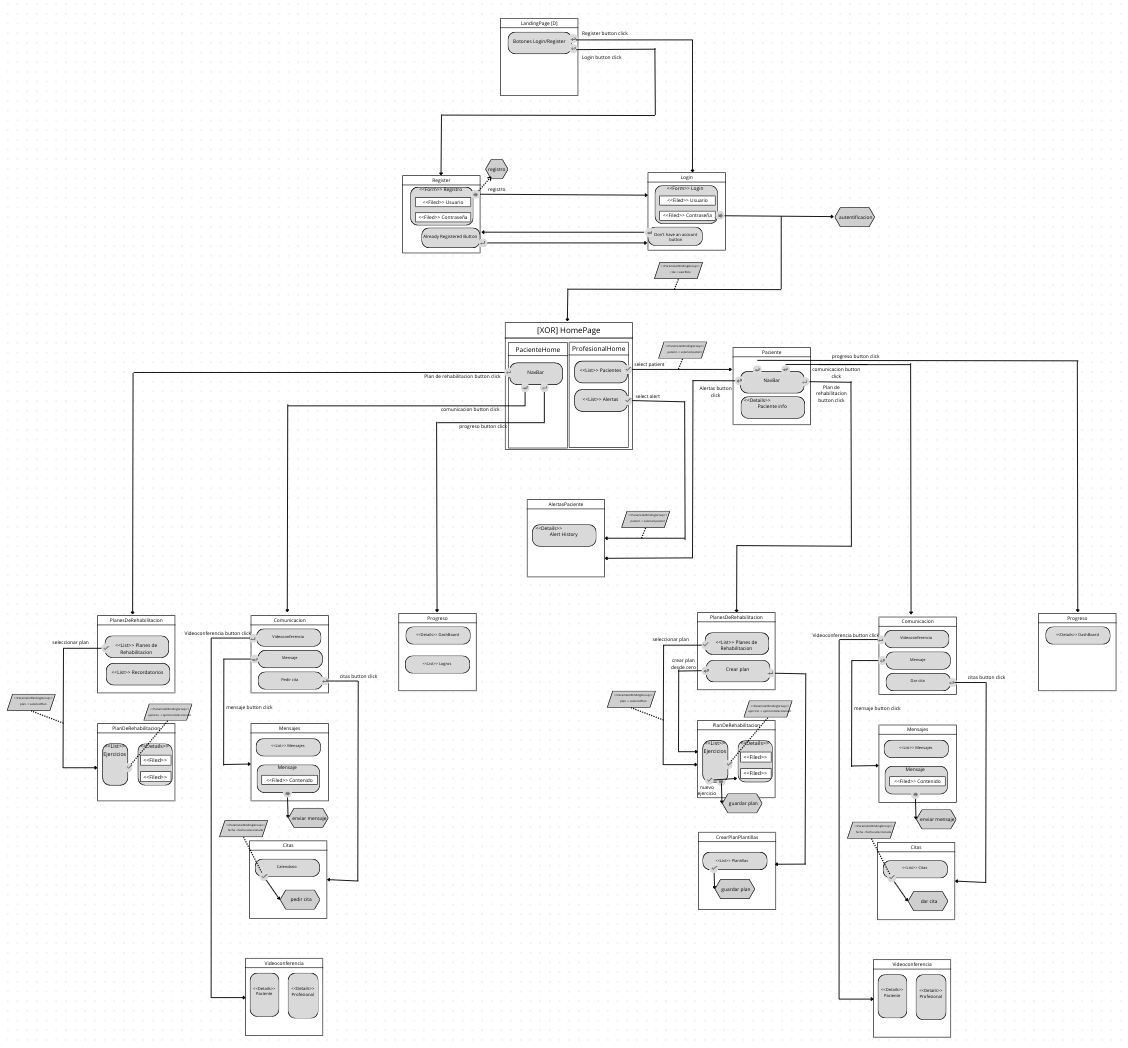
\includegraphics[width=\textwidth]{images/ifml_general.png}
	\caption{Esquema general del modelo IFML para la plataforma. Debido a la complejidad del diagrama, algunos detalles pueden no ser fácilmente visibles.}
	\label{fig:ifml_general}
\end{figure}

La Figura \ref{fig:ifml_general} muestra un esquema general del flujo de interacción en la plataforma. A continuación, se describen más detalladamente algunos de los componentes clave.
\newpage
\subsubsection{Login y Registro}

El proceso de autenticación es uno de los elementos clave en la plataforma. La Figura \ref{fig:ifml_login} ilustra las interacciones del usuario durante el proceso de login y registro, donde los usuarios pueden acceder al sistema como pacientes o profesionales sanitarios.

\begin{figure}[H]
	\centering
	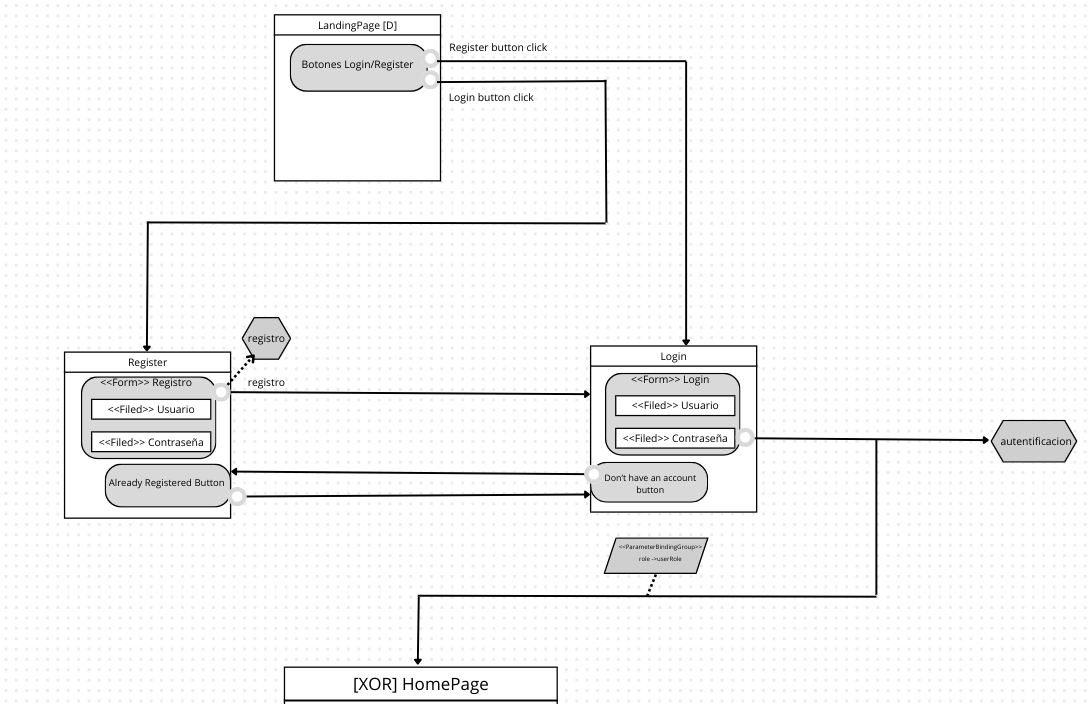
\includegraphics[width=0.8\textwidth]{images/ifml_login.png}
	\caption{IFML del proceso de login y registro de usuarios.}
	\label{fig:ifml_login}
\end{figure}

\subsubsection{Interacciones en el Home}

Dependiendo del tipo de usuario, la plataforma redirige a distintas vistas tras el login. En la Figura \ref{fig:ifml_home}, se muestra cómo un paciente es dirigido a su pantalla principal, mientras que un profesional sanitario tiene acceso a una interfaz diferente con funcionalidades específicas.

\begin{figure}[H]
	\centering
	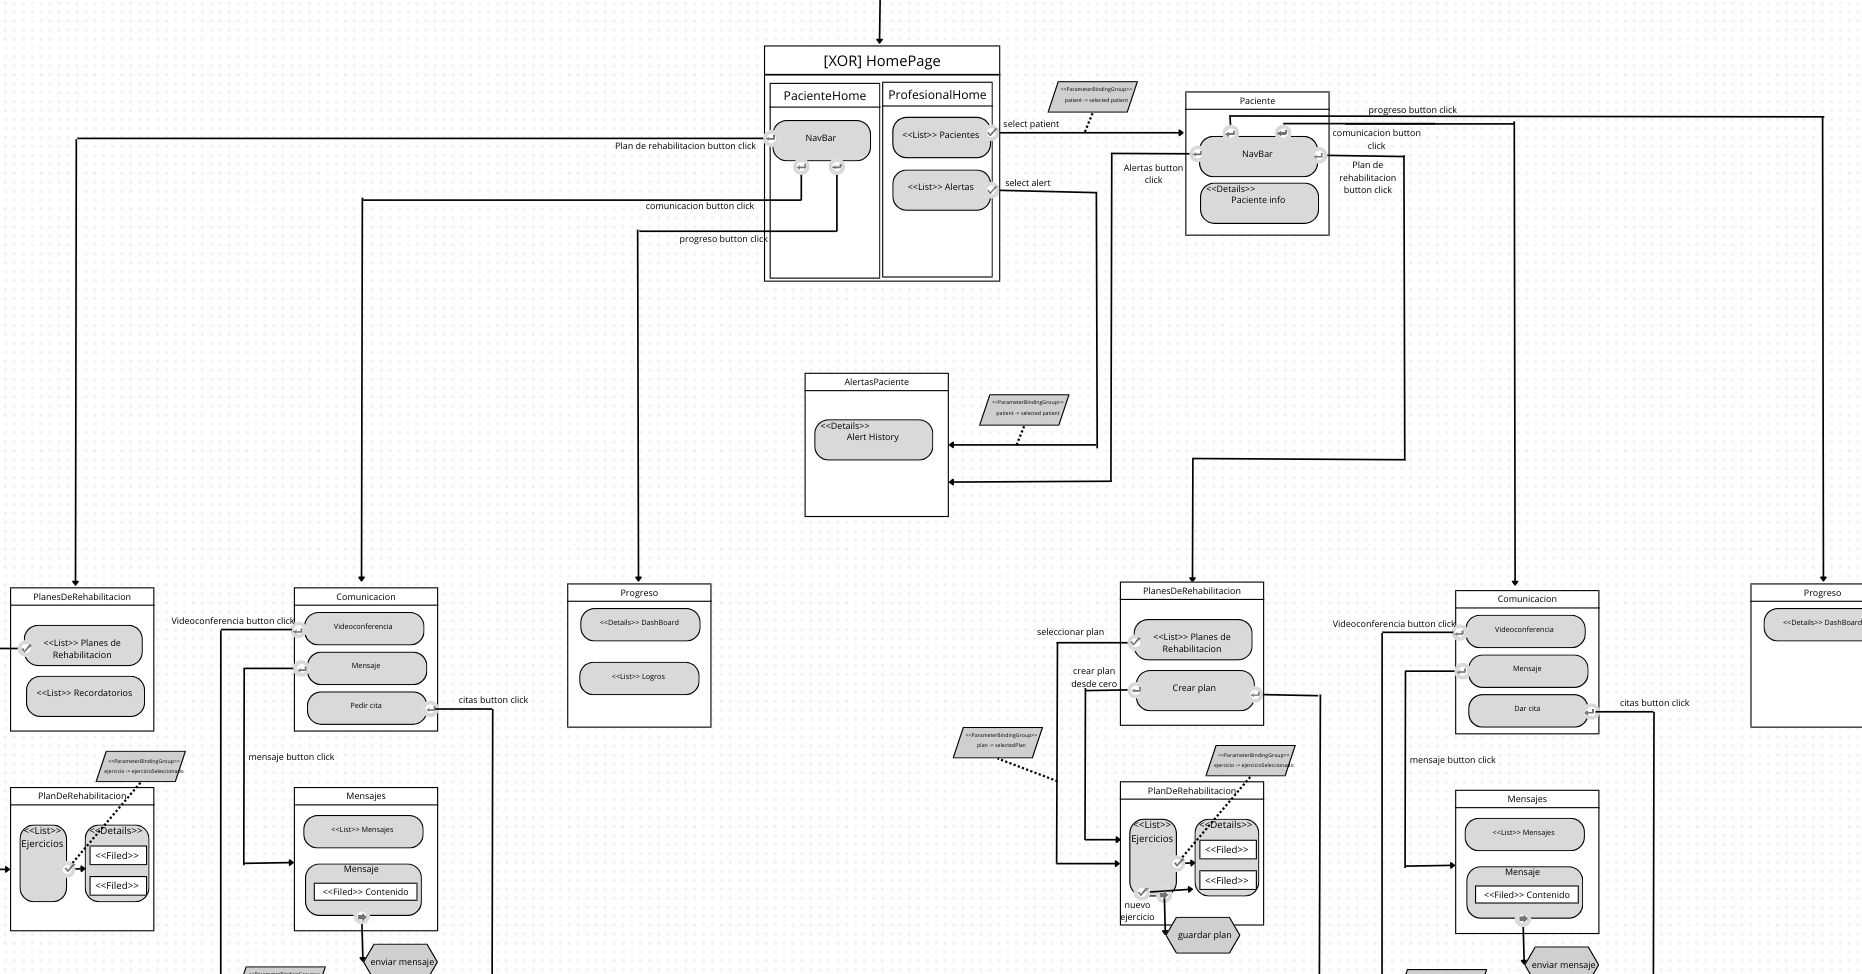
\includegraphics[width=0.8\textwidth]{images/ifml_home.png}
	\caption{IFML de las pantallas de inicio para paciente y profesional sanitario.}
	\label{fig:ifml_home}
\end{figure}

\subsubsection{Interacciones del Paciente}

En la Figura \ref{fig:ifml_paciente}, se detallan todas las posibles interacciones de un paciente dentro de la plataforma, incluyendo la realización de ejercicios, la consulta de informes médicos y la posibilidad de comunicarse con su profesional de la salud.

\begin{figure}[H]
	\centering
	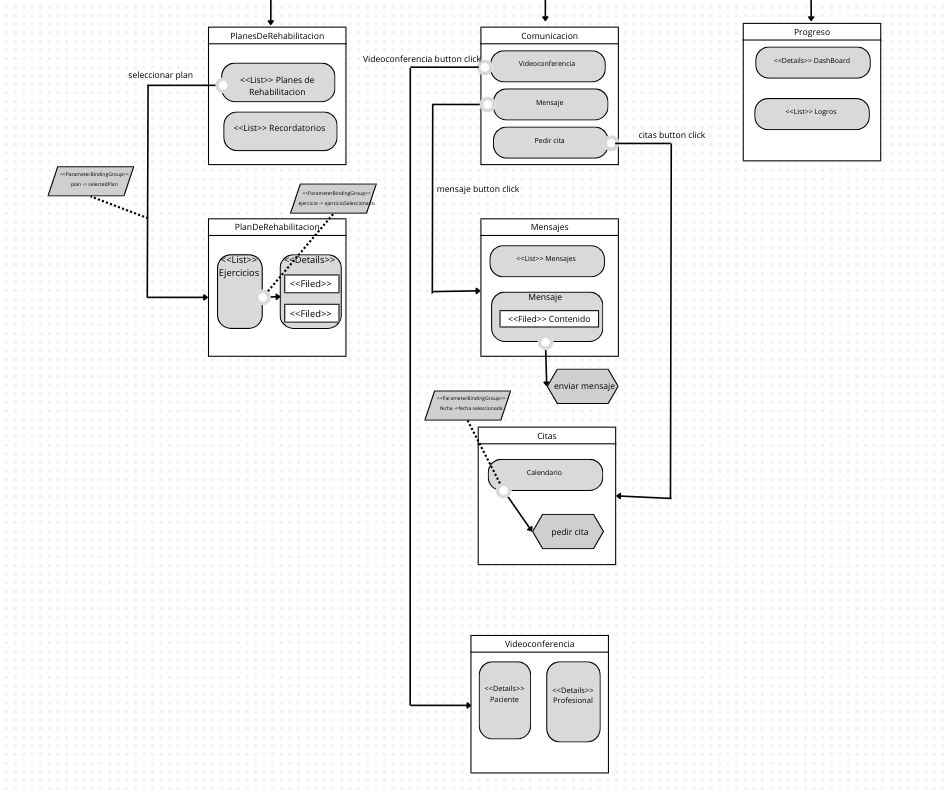
\includegraphics[width=0.8\textwidth]{images/ifml_paciente.png}
	\caption{IFML detallado de las interacciones del paciente.}
	\label{fig:ifml_paciente}
\end{figure}
\newpage
\subsubsection{Interacciones del Profesional Sanitario}

Finalmente, la Figura \ref{fig:ifml_profesional} presenta todas las posibles acciones que un profesional sanitario puede llevar a cabo, tales como la gestión de pacientes, la revisión de informes de rehabilitación y la asignación de nuevos ejercicios.

\begin{figure}[H]
	\centering
	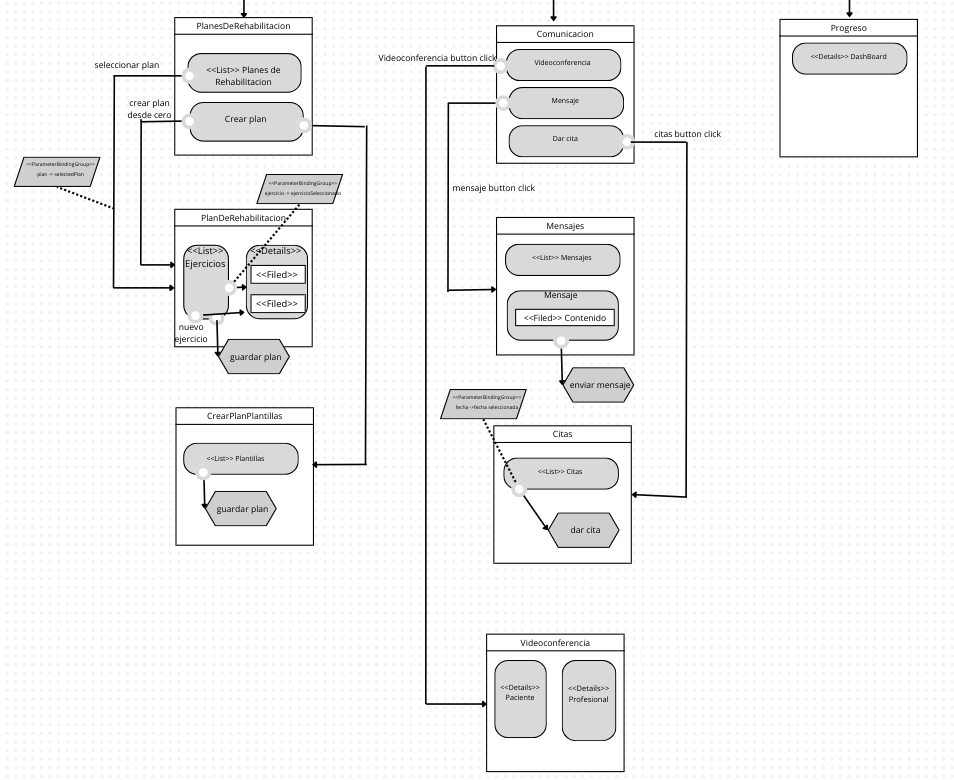
\includegraphics[width=0.8\textwidth]{images/ifml_profesional.png}
	\caption{IFML detallado de las interacciones del profesional sanitario.}
	\label{fig:ifml_profesional}
\end{figure}

Cada uno de estos diagramas IFML ayuda a representar los flujos de interacción específicos para cada tipo de usuario, facilitando la comprensión de los distintos escenarios de uso en la plataforma de telerehabilitación.

\subsection{Diagrama de Clases}

En el desarrollo de software orientado a objetos, el diagrama de clases es una herramienta esencial para representar la estructura del sistema. Este diagrama nos permite modelar las clases principales que intervienen en la aplicación, sus atributos y métodos, así como las relaciones entre ellas. El objetivo es tener una visión clara de cómo se organizan los datos y cómo interactúan los diferentes componentes en el sistema. 

\begin{figure}
	\begin{center} 
		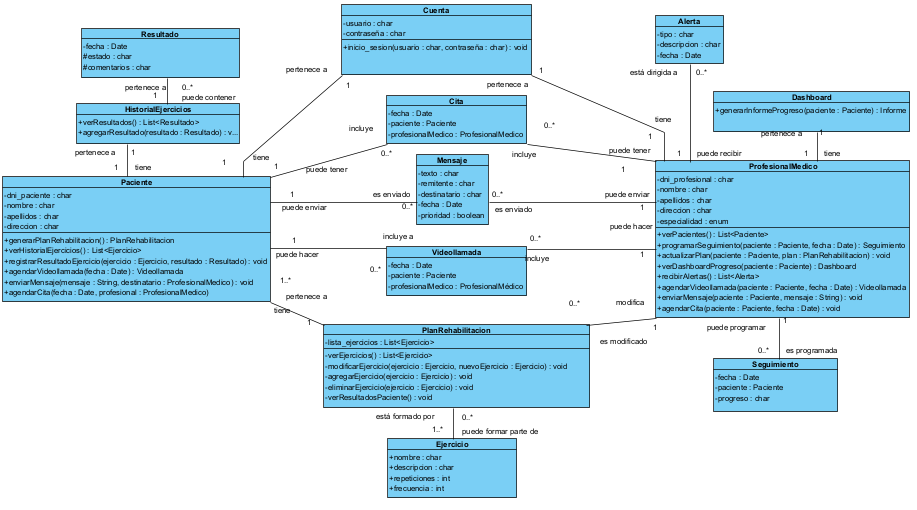
\includegraphics[width=1\textwidth]{images/diagrama_clases.png}
		\caption{Diseño de Diagrama de clases}
		\label{fig:DiagClases}
	\end{center}
\end{figure}
\vspace{5cm}


\subsubsection*{Clases y Métodos de la Aplicación de Rehabilitación}

\subsubsection*{Paciente}

Atributos: \textit{dni\_paciente}, \textit{nombre}, \textit{apellidos}, \textit{direccion}.

Esta entidad mostrará las funciones a las que puede acceder desde la aplicación iniciando sesión como paciente.

\begin{itemize}
	\item \textbf{generarPlanRehabilitacion() : PlanRehabilitacion}  
	Genera un plan de rehabilitación personalizado para el paciente, que incluye los ejercicios y rutinas recomendadas para su recuperación.
	
	\item \textbf{verHistorialEjercicios() : List<Ejercicio>}  
	Permite al paciente ver el historial de ejercicios que ha realizado o que se le han asignado, mostrando información como repeticiones, frecuencia, etc.
	
	\item \textbf{registrarResultadoEjercicio(ejercicio: Ejercicio, resultado: Resultado)}  
	El paciente registra los resultados de un ejercicio específico, incluyendo si completó las repeticiones y cualquier otro dato relevante.
	
	\item \textbf{agendarVideollamada(fecha: Date) : Videollamada}  
	Permite al paciente agendar una videollamada con un profesional médico en una fecha específica.
	
	\item \textbf{enviarMensaje(mensaje: String, destinatario: ProfesionalMedico)}  
	El paciente puede enviar un mensaje al profesional médico dentro de la plataforma para resolver dudas o hacer consultas.
	
	\item \textbf{agendarCita(fecha: Date, profesional: ProfesionalMedico)}  
	Permite al paciente agendar una cita presencial o virtual con un profesional médico en una fecha específica.
\end{itemize}

\subsubsection*{ProfesionalMedico}
Atributos: \textit{dni\_profesional}, \textit{nombre}, \textit{apellidos}, \textit{direccion}, \textit{especialidad}.

Esta entidad mostrará las funciones a las que puede acceder desde la aplicación iniciando sesión como profesional médico.

\begin{itemize}
	\item \textbf{verPacientes() : List<Paciente>}  
	Muestra una lista de los pacientes registrados en la aplicación, con acceso a sus planes de rehabilitación y progreso.
	
	\item \textbf{programarSeguimiento(paciente: Paciente, fecha: Date) : Seguimiento}  
	Permite al profesional médico programar una sesión de seguimiento con un paciente para revisar su progreso.
	
	\item \textbf{actualizarPlan(paciente: Paciente, plan: PlanRehabilitacion)}  
	Actualiza el plan de rehabilitación de un paciente, permitiendo modificar los ejercicios o las rutinas según sea necesario.
	
	\item \textbf{verDashboardProgreso(paciente: Paciente) : Dashboard}  
	Accede a un tablero de control con el progreso del paciente, como resultados de ejercicios, cumplimiento de metas y otros indicadores.
	
	\item \textbf{recibirAlertas() : List<Alerta>}  
	Permite al profesional recibir alertas relacionadas con sus pacientes, como recordatorios o notificaciones sobre problemas en el progreso.
	
	\item \textbf{agendarVideollamada(paciente: Paciente, fecha: Date) : Videollamada}  
	Permite al profesional médico agendar una videollamada con un paciente en una fecha específica.
	
	\item \textbf{enviarMensaje(paciente: Paciente, mensaje: String)}  
	El profesional médico puede enviar mensajes a sus pacientes para dar seguimiento o brindar instrucciones adicionales.
	
	\item \textbf{agendarCita(paciente: Paciente, fecha: Date)}  
	El profesional médico puede agendar citas para una consulta presencial o virtual con el paciente en una fecha específica.
\end{itemize}

\subsubsection*{PlanRehabilitacion}
Atributos: \textit{lista\_ejercicios}.
\begin{itemize}
	\item \textbf{verEjercicios() : List<Ejercicio>}  
	Muestra una lista de todos los ejercicios que forman parte del plan de rehabilitación.
	
	\item \textbf{modificarEjercicio(ejercicio: Ejercicio, nuevoEjercicio: Ejercicio)}  
	Permite modificar un ejercicio en el plan de rehabilitación, cambiando sus características como repeticiones, frecuencia, etc.
	
	\item \textbf{agregarEjercicio(ejercicio: Ejercicio)}  
	Añade un nuevo ejercicio al plan de rehabilitación del paciente.
	
	\item \textbf{eliminarEjercicio(ejercicio: Ejercicio)}  
	Elimina un ejercicio del plan de rehabilitación del paciente.
\end{itemize}

\subsubsection*{Cuenta}
Atributos: \textit{lista\_ejercicios}.
Representa la entidad encargada de gestionar la autenticación de los usuarios, tanto pacientes como profesionales médicos, en la aplicación.
\begin{itemize}
	\item \textbf{inicio\_sesion(usuario : char, contraseña : char) : void}
	Este método verifica si las credenciales proporcionadas (usuario y contraseña) son correctas y permiten el acceso al sistema. Si las credenciales coinciden con las almacenadas, se concede el acceso al usuario. De lo contrario, se rechaza la autenticación y se notificará al usuario que las credenciales son incorrectas.
\end{itemize}

\subsubsection*{Ejercicio}
Atributos: \textit{nombre}, \textit{descripcion}, \textit{repeticiones}, \textit{frecuencia}.  
Los ejercicios contienen información relevante sobre las repeticiones, frecuencia y una descripción detallada del movimiento o acción a realizar.

\subsubsection*{HistorialEjercicios}
\begin{itemize}
	\item \textbf{verResultados() : List<Resultado>}  
	Muestra los resultados obtenidos por el paciente en los ejercicios realizados, con detalle del estado y comentarios.
	
	\item \textbf{agregarResultado(resultado: Resultado)}  
	Agrega un nuevo resultado al historial de ejercicios, almacenando detalles sobre la fecha y el estado del ejercicio.
\end{itemize}

\subsubsection*{Resultado}
Atributos: \textit{fecha}, \textit{estado}, \textit{comentarios}.  
Guarda información sobre el desempeño de un paciente en un ejercicio específico, incluyendo la fecha en que se realizó, el estado del ejercicio (completado o incompleto) y cualquier comentario adicional.

\subsubsection*{Videollamada}
Atributos: \textit{fecha}, \textit{paciente}, \textit{profesionalMedico}.  
Almacena la información de una videollamada programada, como la fecha y los participantes (paciente y profesional médico).

\subsubsection*{Mensaje}
Atributos: \textit{texto}, \textit{remitente}, \textit{destinatario}, \textit{fecha}, \textit{prioridad}.  
Un mensaje enviado entre un paciente y un profesional médico, con detalles sobre el contenido, remitente, destinatario, la fecha de envío y si es prioritario o no.

\subsubsection*{Cita}
Atributos: \textit{fecha}, \textit{paciente}, \textit{profesionalMedico}.  
Guarda la información de una cita programada, ya sea presencial o virtual, entre un paciente y un profesional médico.

\subsubsection*{Seguimiento}
Atributos: \textit{fecha}, \textit{paciente}, \textit{progreso}.  
Registra los detalles de una sesión de seguimiento, incluyendo la fecha, el paciente y el progreso discutido o observado durante la sesión.

\subsubsection*{Dashboard}
\begin{itemize}
	\item \textbf{generarInformeProgreso(paciente: Paciente) : Informe}  
	Genera un informe detallado del progreso del paciente, basado en sus resultados, ejercicios realizados y cumplimiento de objetivos.
\end{itemize}

\subsubsection*{Alerta}
Atributos: \textit{tipo}, \textit{descripcion}, \textit{fecha}.  
Contiene información sobre una alerta que puede estar relacionada con citas próximas, tareas incompletas o actualizaciones en el plan de rehabilitación.

\subsubsection*{Clases y Relaciones con Multiplicidades}

\begin{itemize}
	\item \textbf{Paciente}
	\begin{itemize}
		\item \textbf{PlanRehabilitacion} (1) — Un paciente tiene un plan de rehabilitación.
		\item \textbf{HistorialEjercicios} (1) — Un paciente tiene un historial de ejercicios.
		\item \textbf{Cuenta} (1) — Un paciente tiene una cuenta.
		\item \textbf{Videollamada} (0..*) — Un paciente puede tener cero o muchas videollamadas.
		\item \textbf{Mensaje} (0..*) — Un paciente puede enviar o recibir cero o muchos mensajes.
		\item \textbf{Cita} (0..*) — Un paciente puede tener cero o muchas citas agendadas con un profesional médico.
	\end{itemize}
	
	\item \textbf{Cuenta}
	\begin{itemize}
		\item \textbf{Paciente} (1) — Una cuenta pertenece a un paciente.
		\item \textbf{ProfesionalMedico} (1) — Una cuenta pertenece a un profesional médico.
	\end{itemize}
	\item \textbf{ProfesionalMedico}
	\begin{itemize}
		\item \textbf{Paciente} (1) — Un profesional médico puede atender a cero o muchos pacientes.
		\item \textbf{Cuenta} (1) — Un profesional médico tiene una cuenta.
		\item \textbf{PlanRehabilitacion} (0..*) — Un profesional médico puede modificar los planes de rehabilitación de cero o muchos pacientes.
		\item \textbf{Videollamada} (0..*) — Un profesional médico puede tener cero o muchas videollamadas con pacientes.
		\item \textbf{Mensaje} (0..*) — Un profesional médico puede enviar o recibir cero o muchos mensajes.
		\item \textbf{Cita} (0..*) — Un profesional médico puede tener cero o muchas citas agendadas con pacientes.
		\item \textbf{Seguimiento} (0..*) — Un profesional médico puede programar cero o muchas sesiones de seguimiento para pacientes.
		\item \textbf{Dashboard} (1) — Un profesional médico tiene un dashboard de progreso para cada paciente que sigue.
		\item \textbf{Alerta} (0..*) — Un profesional médico puede recibir cero o muchas alertas relacionadas con los pacientes.
	\end{itemize}
	
	\item \textbf{PlanRehabilitacion}
	\begin{itemize}
		\item \textbf{Ejercicio} (1..*) — Un plan de rehabilitación debe tener al menos un ejercicio.
		\item \textbf{Paciente} (1) — Un plan de rehabilitación pertenece a exactamente un paciente.
	\end{itemize}
	
	\item \textbf{Ejercicio}
	\begin{itemize}
		\item \textbf{PlanRehabilitacion} (1) — Cada ejercicio pertenece a exactamente un plan de rehabilitación.
	\end{itemize}
	
	\item \textbf{HistorialEjercicios}
	\begin{itemize}
		\item \textbf{Resultado} (0..*) — Un historial de ejercicios puede contener cero o muchos resultados de los ejercicios realizados.
		\item \textbf{Paciente} (1) — Un historial de ejercicios pertenece a exactamente un paciente.
	\end{itemize}
	
	\item \textbf{Resultado}
	\begin{itemize}
		\item \textbf{Ejercicio} (1) — Un resultado pertenece a exactamente un ejercicio.
		\item \textbf{HistorialEjercicios} (1) — Un resultado pertenece a exactamente un historial de ejercicios.
	\end{itemize}
	
	\item \textbf{Videollamada}
	\begin{itemize}
		\item \textbf{Paciente} (1) — Cada videollamada incluye a exactamente un paciente.
		\item \textbf{ProfesionalMedico} (1) — Cada videollamada incluye a exactamente un profesional médico.
	\end{itemize}
	
	\item \textbf{Mensaje}
	\begin{itemize}
		\item \textbf{Paciente} (1) — Cada mensaje es enviado o recibido por exactamente un paciente.
		\item \textbf{ProfesionalMedico} (1) — Cada mensaje es enviado o recibido por exactamente un profesional médico.
	\end{itemize}
	
	\item \textbf{Cita}
	\begin{itemize}
		\item \textbf{Paciente} (1) — Cada cita incluye a exactamente un paciente.
		\item \textbf{ProfesionalMedico} (1) — Cada cita incluye a exactamente un profesional médico.
	\end{itemize}
	
	\item \textbf{Seguimiento}
	\begin{itemize}
		\item \textbf{Paciente} (1) — Cada seguimiento está asociado a exactamente un paciente.
		\item \textbf{ProfesionalMedico} (1) — Cada seguimiento está asociado a exactamente un profesional médico.
	\end{itemize}
	
	\item \textbf{Dashboard}
	\begin{itemize}
		\item \textbf{Paciente} (1) — Un dashboard de progreso está asociado a exactamente un paciente.
		\item \textbf{ProfesionalMedico} (1) — Un dashboard de progreso pertenece a exactamente un profesional médico.
	\end{itemize}
	
	\item \textbf{Alerta}
	\begin{itemize}
		\item \textbf{ProfesionalMedico} (1) — Cada alerta está dirigida a exactamente un profesional médico.
	\end{itemize}
\end{itemize}


\end{document}
